\section{Results and discussion}
\subsection{Effect of operating temperature on water flow rate outflow from air side}

Figure \ref{fig:fig5} shows the change in the water flow out of the air side at different working temperatures. As can be seen from the figure \ref{fig:fig5a}, as the temperature rises, the water content in the air side exhaust gas generally shows an upward trend. The higher the temperature, the higher the saturation vapor pressure of the fuel cell. Under the same water content, the relative humidity will decrease at this time, which is equivalent to the generation of less liquid water inside the fuel cell, and the ability of the gas to carry water is improved. This change applies to both the air side and the hydrogen side, which is shown in figure \ref{fig:figure4b} and figure \ref{fig:figure4c}. Therefore, under the same other conditions, the water flow out of the fuel cell stack by the air increases with the increase in temperature, and more liquid water is collected by the air side exhaust gas collection device.
% 图\ref{fig:fig5}显示了不同工作温度下空气侧流出水流量的变化。 从图\ref{fig:fig5}(a)可以看出,随着温度的升高,空气侧废气中的含水量总体呈上升趋势。 温度越高,燃料电池的饱和蒸气压越高。 相同含水量下,此时相对湿度会降低,相当于燃料电池内部产生的液态水较少,气体携带水的能力提高。 这种变化适用于空气侧和氢气侧,如图(b)和图(c)所示。 因此,在其他条件相同的情况下,空气从燃料电池堆流出的水量随着温度的升高而增加,空气侧废气收集装置收集到更多的液态水。
\par
It is worth noting that when the load current is 120A, the impact of the working temperature on the water flow of the air side is slightly different under different metering ratios. As the air metering ratio increases, the growth rate of the water flow on the air side gradually decreases. This is because at a small current density, the fuel cell produces less water due to the electrochemical reaction, and at the same time, the high-speed high-temperature reaction gas has a strong ability to carry water, and the water produced by the fuel cell has been completely carried out by the reaction gas. Therefore, even if the air metering ratio increases, the reaction gas cannot carry out more water. For the working conditions of low working temperature and large load current, the ability of the reaction gas to carry water is low or the fuel cell produces more water, so there is still some water vapor or liquid water remaining in the system. At this time, if the air flow is increased, the water flow out of the system will also increase accordingly.
% 值得注意的是,负载电流为120A时,不同计量比下工作温度对空气侧水流量的影响略有不同。 随着空气计量比的增大,空气侧水流量的增长率逐渐减小。 这是因为在较小的电流密度下,燃料电池因电化学反应产生的水较少,同时高速高温反应气体具有很强的携带水的能力,燃料电池产生的水 燃料电池的反应已完全由气体进行。 因此,即使空气计量比增大,反应气体也不能带出更多的水。 对于工作温度低、负载电流大的工况,反应气体携带水的能力较低或燃料电池产生的水较多,因此系统中仍残留有一些水蒸气或液态水。 此时,如果空气流量增加,则系统流出的水流量也会相应增加。
\subfile{Airside_Waterflow_figure_1.tex}
\par
Fig \ref{fig:fig5a} shows that as the temperature rises, the water content in the hydrogen side exhaust gas generally shows a downward trend, and even at 120A/70$^{\circ}C$, the water content in the hydrogen side exhaust gas is 0, the same result appears in 210A(fig \ref{fig:fig5c}) and 300A(fig \ref{fig:fig5c}). There are mainly two reasons for this phenomenon.  First, according to the principle of proton exchange membrane fuel cell reaction, the reaction product water is generated at the cathode (that is, the air side), and the fuel used by the fuel cell system is 99.99\% pure hydrogen. Therefore, the water inside the hydrogen side is mainly the water that migrates from the air side to the hydrogen side under the action of concentration diffusion and pressure diffusion. Since the hydrogen-air pressure difference is basically consistent (20kpa) during the experiment, the influence of pressure on water migration can be ignored when comparing. Second, the exhaust gas collected on the anode side needs to first pass through the water separator built into the fuel cell system to separate the unreacted hydrogen from the liquid water, and then it can be collected by the exhaust water collection device on the hydrogen side. And at higher working temperatures, the saturation vapor pressure of the gas on the hydrogen side rises, and the content of liquid water decreases relatively. These two factors cause the working temperature to rise and the water content flowing out of the hydrogen side to decrease.
% 由图\ref{fig:fig5}(a)可知,随着温度的升高,氢侧废气中的水含量总体呈下降趋势,即使在120A/70$^{\circ}C$下,水含量也呈下降趋势。 当氢气侧废气中的含量为0时,210A(fig \ref{fig:fig5}(c))和300A(fig \ref{fig:fig5}(c))中出现相同的结果。 造成这种现象的原因主要有两个。 首先,根据质子交换膜燃料电池反应原理,在阴极(即空气侧)生成反应产物水,燃料电池系统使用的燃料为99.99%的纯氢气。 因此,氢气侧内部的水主要是在浓度扩散和压力扩散的作用下从空气侧迁移到氢气侧的水。 由于实验过程中氢气与空气的压差基本一致(20kpa),因此比较时可以忽略压力对水迁移的影响。 其次,阳极侧收集的废气首先需要经过燃料电池系统内置的水分离器,将未反应的氢气与液态水分离,然后可由氢气侧的废气水收集装置收集 。 并且在较高的工作温度下,氢侧气体的饱和蒸气压升高,液态水的含量相对减少。 这两个因素导致工作温度升高,氢气侧流出的含水量减少。

\subfile{Airside_Waterflow_figure_2.tex}

\subsection{Influence of air metering ratio on the water flow out of the cathode and anode}

Compare the water flow out of the air side and the hydrogen side at 120A, 210A, 300A load currents, different coolant inlet temperatures, and different air metering ratios, as shown in Fig \ref{fig:figure6a}. Similar to the impact of working temperature on the water flow out of the air side, under the same load current, the higher the air metering ratio, the more water is carried out of the stack by the unreacted air, which also applies to load current of 210A(fig \ref{fig:figure6b}) and 300A(fig \ref{fig:figure6c}). It should be noted that this growth is not unlimited. After reaching a certain air metering ratio, the growth of the water content in the air side exhaust gas slows down, especially when the load current is small and the working temperature is high. This is because at this time, the water produced by the electrochemical reaction of the fuel cell has been completely carried out of the fuel cell by high-temperature high-speed air. At this time, even if the air metering ratio continues to increase, the water content of the exhaust gas will not continue to increase.
% 比较120A、210A、300A负载电流、不同冷却液入口温度、不同空气计量比下空气侧和氢气侧流出的水流量,如图\ref{figure6}(a)所示。 与工作温度对空气侧水流量的影响类似,在相同的负载电流下,空气计量比越高,未反应的空气带出电堆的水就越多,这也适用于负载电流 210A(图\ref{图6}(b))和300A(图\ref{图6}(c))。 值得注意的是,这种增长并不是无限的。 达到一定的空气计量比后,空气侧废气中含水量的增长减慢,特别是在负载电流较小、工作温度较高时。 这是因为此时燃料电池电化学反应产生的水已经被高温高速空气完全带出燃料电池。 此时,即使空气计量比继续增加,废气的含水量也不会继续增加。
\subfile{Airside_Waterflow_figure_grouped_by_temperature.tex}
\par
For the hydrogen side, similarly, as the air metering ratio increases, the water flow out of the hydrogen side basically continues to decrease. After the above analysis, as the air metering ratio increases, the water stored in the cathode will be taken out of the stack by the high-speed airflow, and the water flow diffused to the hydrogen side through concentration difference becomes less, so relatively speaking, the water collected on the hydrogen side will become less. However, the degree of decline is different. Under low temperature (120A/60$^{\circ}C$, 210A/60$^{\circ}C$, and 300A/63$^{\circ}C$), they all show a relatively gentle decline. As the temperature rises, the water flow out of the hydrogen side is also gradually affected by the air metering ratio.
% 对于氢气侧,同样,随着空气计量比的增大,氢气侧流出的水流量基本持续减少。 经过上述分析,随着空气计量比的增大,储存在阴极的水会被高速气流带出电堆,通过浓度差扩散到氢气侧的水流量变少,所以相对而言 ,氢气侧收集的水会变少。 但下降的程度不同。 在低温下(120A/60$^{\circ}C$、210A/60$^{\circ}C$、300A/63$^{\circ}C$),它们都表现出相对平缓的下降。 随着温度的升高,氢气侧流出的水量也逐渐受到空气计量比的影响。

\subfile{Hydroside_Waterflow_figure_grouped_by_temperature.tex}

\subsection{Effects of operating temperature and air metering ratio on internal water content of fuel cell system}
According to the working principle of the fuel cell, during the reaction process, water mainly comes from the electrochemical reaction and the water vapor that enters the fuel cell with the reaction gas. Then, a part of the water is discharged from the fuel cell with the exhaust gas after the reaction, and another part of the water stays inside the fuel cell. In this article, the change rate of the water remaining in the fuel cell will be used as the research object to evaluate the water content status inside the fuel cell.
% 根据燃料电池的工作原理,在反应过程中,水主要来自于电化学反应以及随反应气体进入燃料电池的水蒸气。 然后,反应后一部分水随废气一起从燃料电池中排出,另一部分水留在燃料电池内部。 本文将以燃料电池中残留水的变化率作为研究对象来评估燃料电池内部的含水量状况。
\begin{equation}
	\label{eq9}
	{\frac{d m_{w,s t k}}{d t}}=Q_{w,i n,s y s}+Q_{w,g e n}-Q_{w,o u t,c a}-Q_{w,o u t,a n}
\end{equation}
In formula \ref{eq9}, $m_(w,stk)$ is the water content inside the fuel cell, in g, $Q_(w,in,sys)$ is the water flow rate entering the fuel cell system, in (g/s), $Q_(w,gen)$ represents the water flow rate generated by the electrochemical reaction, in (g/s), $Q_(w,out,ca)$ represents the water flow rate flowing out of the system from the cathode, in (g/s), $Q_(w,out,an)$ represents the water flow rate flowing out of the system from the anode, in (g/s).
% 式\ref{eq9}中,$m_(w,stk)$为燃料电池内部的水含量,单位为g,$Q_(w,in,sys)$为进入燃料电池系统的水流量,单位为g (g/s),$Q_(w,gen)$表示电化学反应产生的水流量,单位(g/s),$Q_(w,out,ca)$表示流出的水流量 $Q_(w,out,an)$表示从阳极流出系统的水流量,单位(g/s),$Q_(w,out,an)$表示从阳极流出系统的水流量,单位(g/s)。
\par
Although during the reaction process, under the effects of concentration diffusion and electro-osmotic drag, water at the cathode will migrate to the anode. However, the research object of the water balance method is the entire fuel cell, so the internal water migration process will not have an impact.
% 虽然在反应过程中,在浓度扩散和电渗阻力的作用下,阴极的水会迁移到阳极。 但水平衡法的研究对象是整个燃料电池,因此内部的水迁移过程不会产生影响。
\par
Using the method described above, the rate of change of the water content inside the fuel cell system under different load currents, working temperatures, and air metering ratios can be calculated. In the process of making the graph, to maintain the integrity of the graph. We use (Load current/Temperature/Coefficient) as the format of test environment description. The data of (210A/55$^{\circ}C$/1.8 ) and (210A/55$^{\circ}C$/2.0) are replaced with (210A/55$^{\circ}C$/2.2) test's data. The obtained results are compared as shown in Fig \ref{fig:fig8a}, Fig \ref{fig:fig8b} and Fig \ref{fig:fig8c}, where positive values indicate an increase in water content (represented in blue), and negative values indicate a decrease in water content (represented in red). For the convenience of subsequent discussions, the blue part is defined as flooding, the red part is defined as drying, and the green part is defined as the normal state.
% 利用上述方法,可以计算出在不同负载电流、工作温度和空气计量比下燃料电池系统内部含水量的变化率。 在制作图表的过程中,要保持图表的完整性。 我们使用(负载电流/温度/系数)作为测试环境描述的格式。 (210A/55$^{\circ}C$/1.8 ) 和 (210A/55$^{\circ}C$/2.0) 的数据替换为 (210A/55$^{\circ}C$/ 2.2) 测试数据。 得到的结果对比如图\ref{fig:fig8a}、Fig \ref{fig:fig8b}和Fig \ref{fig:fig8c}所示,其中正值表示含水量增加(以蓝色表示), 负值表示水分含量减少(以红色表示)。 为了后续讨论方便,蓝色部分定义为泛滥,红色部分定义为干燥,绿色部分定义为正常状态。

\begin{figure}[ht]
	\centering
	\subfloat[\label{fig:fig8a}]{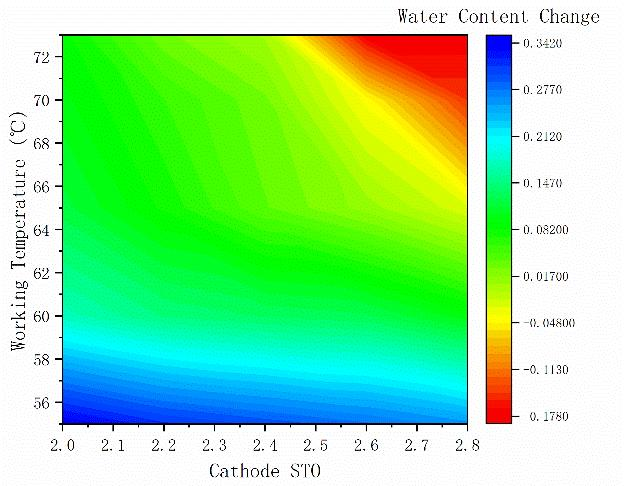
\includegraphics[width=0.4\textwidth]{Research_pictures/fig8a.jpg}}
	\subfloat[\label{fig:fig8b}]{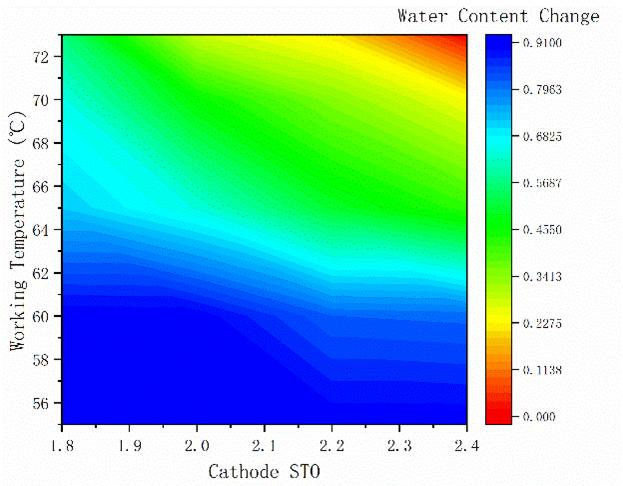
\includegraphics[width=0.4\textwidth]{Research_pictures/fig8b.jpg}}
	\\
	\subfloat[\label{fig:fig8c}]{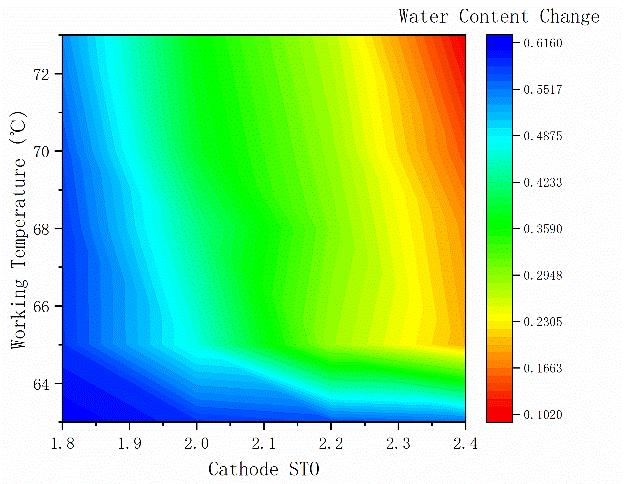
\includegraphics[width=0.4\textwidth]{Research_pictures/fig8c.jpg}}
	\caption{Comparison chart of internal water content of fuel cell system under different conditions (a:120A; b:210A; c:300A)}
	\label{fig:figure8}
\end{figure}

As can be seen from Fig \ref{fig:figure8}, under the same load current, as the working temperature increases and the air metering ratio increases, the rate of change of the water content inside the fuel cell system gradually decreases. When it is 120A/73$^{\circ}C$/2.8, 210A/73$^{\circ}C$/2.4, 300A/73$^{\circ}C$/2.4, the rate of change of the water content inside the fuel cell system reaches the minimum value under this load current. However, the degree of influence of the working temperature and the air metering ratio on the rate of change of the water content inside the fuel cell system is slightly different. When the load current is 120A and 210A, too low working temperature is more likely to cause flooding than too low air metering ratio. For example, at 120A, when the working temperature is 55$^{\circ}C$, even if the air metering ratio reaches 2.8, the fuel cell system is still in a relatively flooded state; and when the working temperature is 73$^{\circ}C$, even if the air metering ratio is only 2.0, the fuel cell system is in a normal state. In a dry state, the degree of influence of working temperature and air metering ratio is not much different. However, when the load current is 310A, the trend is the opposite. Too low working temperature and too low air metering ratio will cause flooding, and too high air metering ratio is more likely to cause drying than too high working temperature.
% 从图\ref{fig:figure8}可以看出,在相同的负载电流下,随着工作温度的升高和空气计量比的增大,燃料电池系统内部含水量的变化率逐渐减小。 当为 120A/73$^{\circ}C$/2.8、210A/73$^{\circ}C$/2.4、300A/73$^{\circ}C$/2.4 时,变化率为 在此负载电流下,燃料电池系统内部的含水量达到最小值。 但工作温度和空气计量比对燃料电池系统内部含水量变化率的影响程度略有不同。 当负载电流为120A、210A时,工作温度过低比空气计量比过低更容易引起水淹。 例如,在120A时,工作温度为55$^{\circ}C$时,即使空气计量比达到2.8,燃料电池系统仍处于相对淹没状态; 当工作温度为73$^{\circ}C$时,即使空气计量比仅为2.0,燃料电池系统也处于正常状态。 在干燥状态下,工作温度和空气计量比的影响程度相差不大。 但当负载电流为310A时,趋势相反。 工作温度过低、空气计量比过低会引起水淹,空气计量比过高比工作温度过高更容易引起干燥。
\par
Furthermore, this paper uses the method of linear regression to analyze the impact of working temperature and air metering ratio on the water content inside the fuel cell system. Before this, the data needs to be standardized. This paper uses the Z-score normalization method\cite{altman2013predicting,camska2013predicting}, which is
% 此外,本文采用线性回归的方法分析了工作温度和空气计量比对燃料电池系统内部含水量的影响。 在此之前,需要对数据进行标准化处理。 本文采用Z-score归一化方法,即
$$x^{*}=x-\mu\sigma$$

\par
Table \ref{tab:RegressionAnalysis} shows the result of analysis:
\begin{table}
	\centering
	\begin{center}
		\caption{Regression analysis under different load current}
		\label{tab:RegressionAnalysis}
		\begin{tabular}{l|l|l}
			\hline
			\textbf{Load current(A)} & \textbf{\makecell{Temperature ratio           \\regression coefficient}} & \textbf{\makecell{Air metering\\ratio regression coefficient}} \\
			\hline
			120                      & -0.8469                             & -0.4145 \\
			210                      & -0.9341                             & -0.4347 \\
			300                      & -0.4637                             & -0.7618 \\
			\hline
		\end{tabular}
	\end{center}
\end{table}
Similar to the phenomenon described above, the impact of the working temperature is more significant when load current is on 120A and 210A; while the impact of the air metering ratio is more significant when load current is 300A. Reason for this phenomenon may be the air metering ratio related to the load current. Under different load currents, the air metering ratio changes the same magnitude, but the change in air flow is different. Since the fuel cell system needs to rely on high-speed high-temperature gas to carry the water out, the higher the load current, the more significant the impact of the air metering ratio.
% 与上述现象类似,负载电流为120A和210A时,工作温度的影响更为显着; 而当负载电流为300A时,空气计量比的影响更为显着。 造成这种现象的原因可能是:空气计量比与负载电流有关。 不同负载电流下,空气计量比变化相同幅度,但风量变化不同。 由于燃料电池系统需要依靠高速高温气体将水带出,负载电流越高,空气计量比的影响越显着。所以,当负载电流升高时,空气计量比的影响更为显着。
\par
Therefore, to maintain the long-term stable operation of the fuel cell system, appropriate operating conditions need to be selected. The following principles should be considered when choosing:
% 因此,为了维持燃料电池系统的长期稳定运行,需要选择合适的运行工况。 选择时应考虑以下原则:
\begin{itemize}
	\item The fuel cell system should be in a normal state under this condition;
	\item In the actual operation process, there are certain fluctuations in the working temperature and air metering ratio. The fluctuation range of the working temperature is about $\pm2^{\circ}C$, and the fluctuation range of the air metering ratio is about$\pm0.1$, so the selected conditions should make the points within the fluctuation range in a normal state;
	\item A larger air metering ratio and a lower working temperature will cause additional consumption of the auxiliary system, so try to choose working conditions with a low air metering ratio and a high working temperature.
\end{itemize}
As shown in Fig \ref{fig:figure9}, 120A/67$^{\circ}C$/2.15, 210A/68$^{\circ}C$/2.15, 300A/70$^{\circ}C$/2.05 are selected as the appropriate operating conditions under each load current.
\begin{figure}[ht]
	\centering
	\subfloat[\label{fig:fig9a}]{
		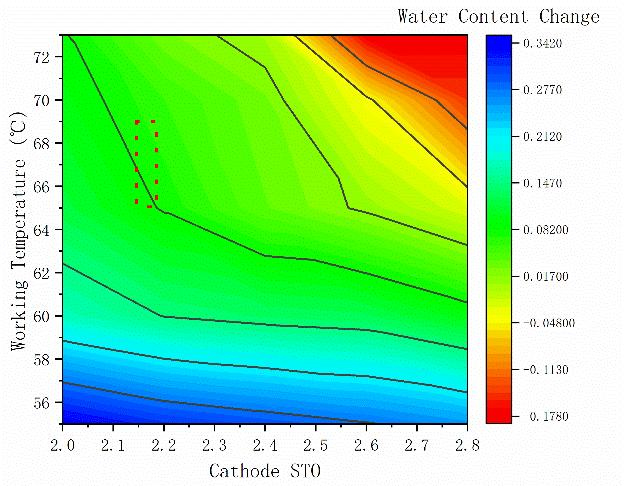
\includegraphics[width=0.5\textwidth]{Research_pictures/fig9a.jpg}
	}
	\subfloat[\label{fig:fig9b}]{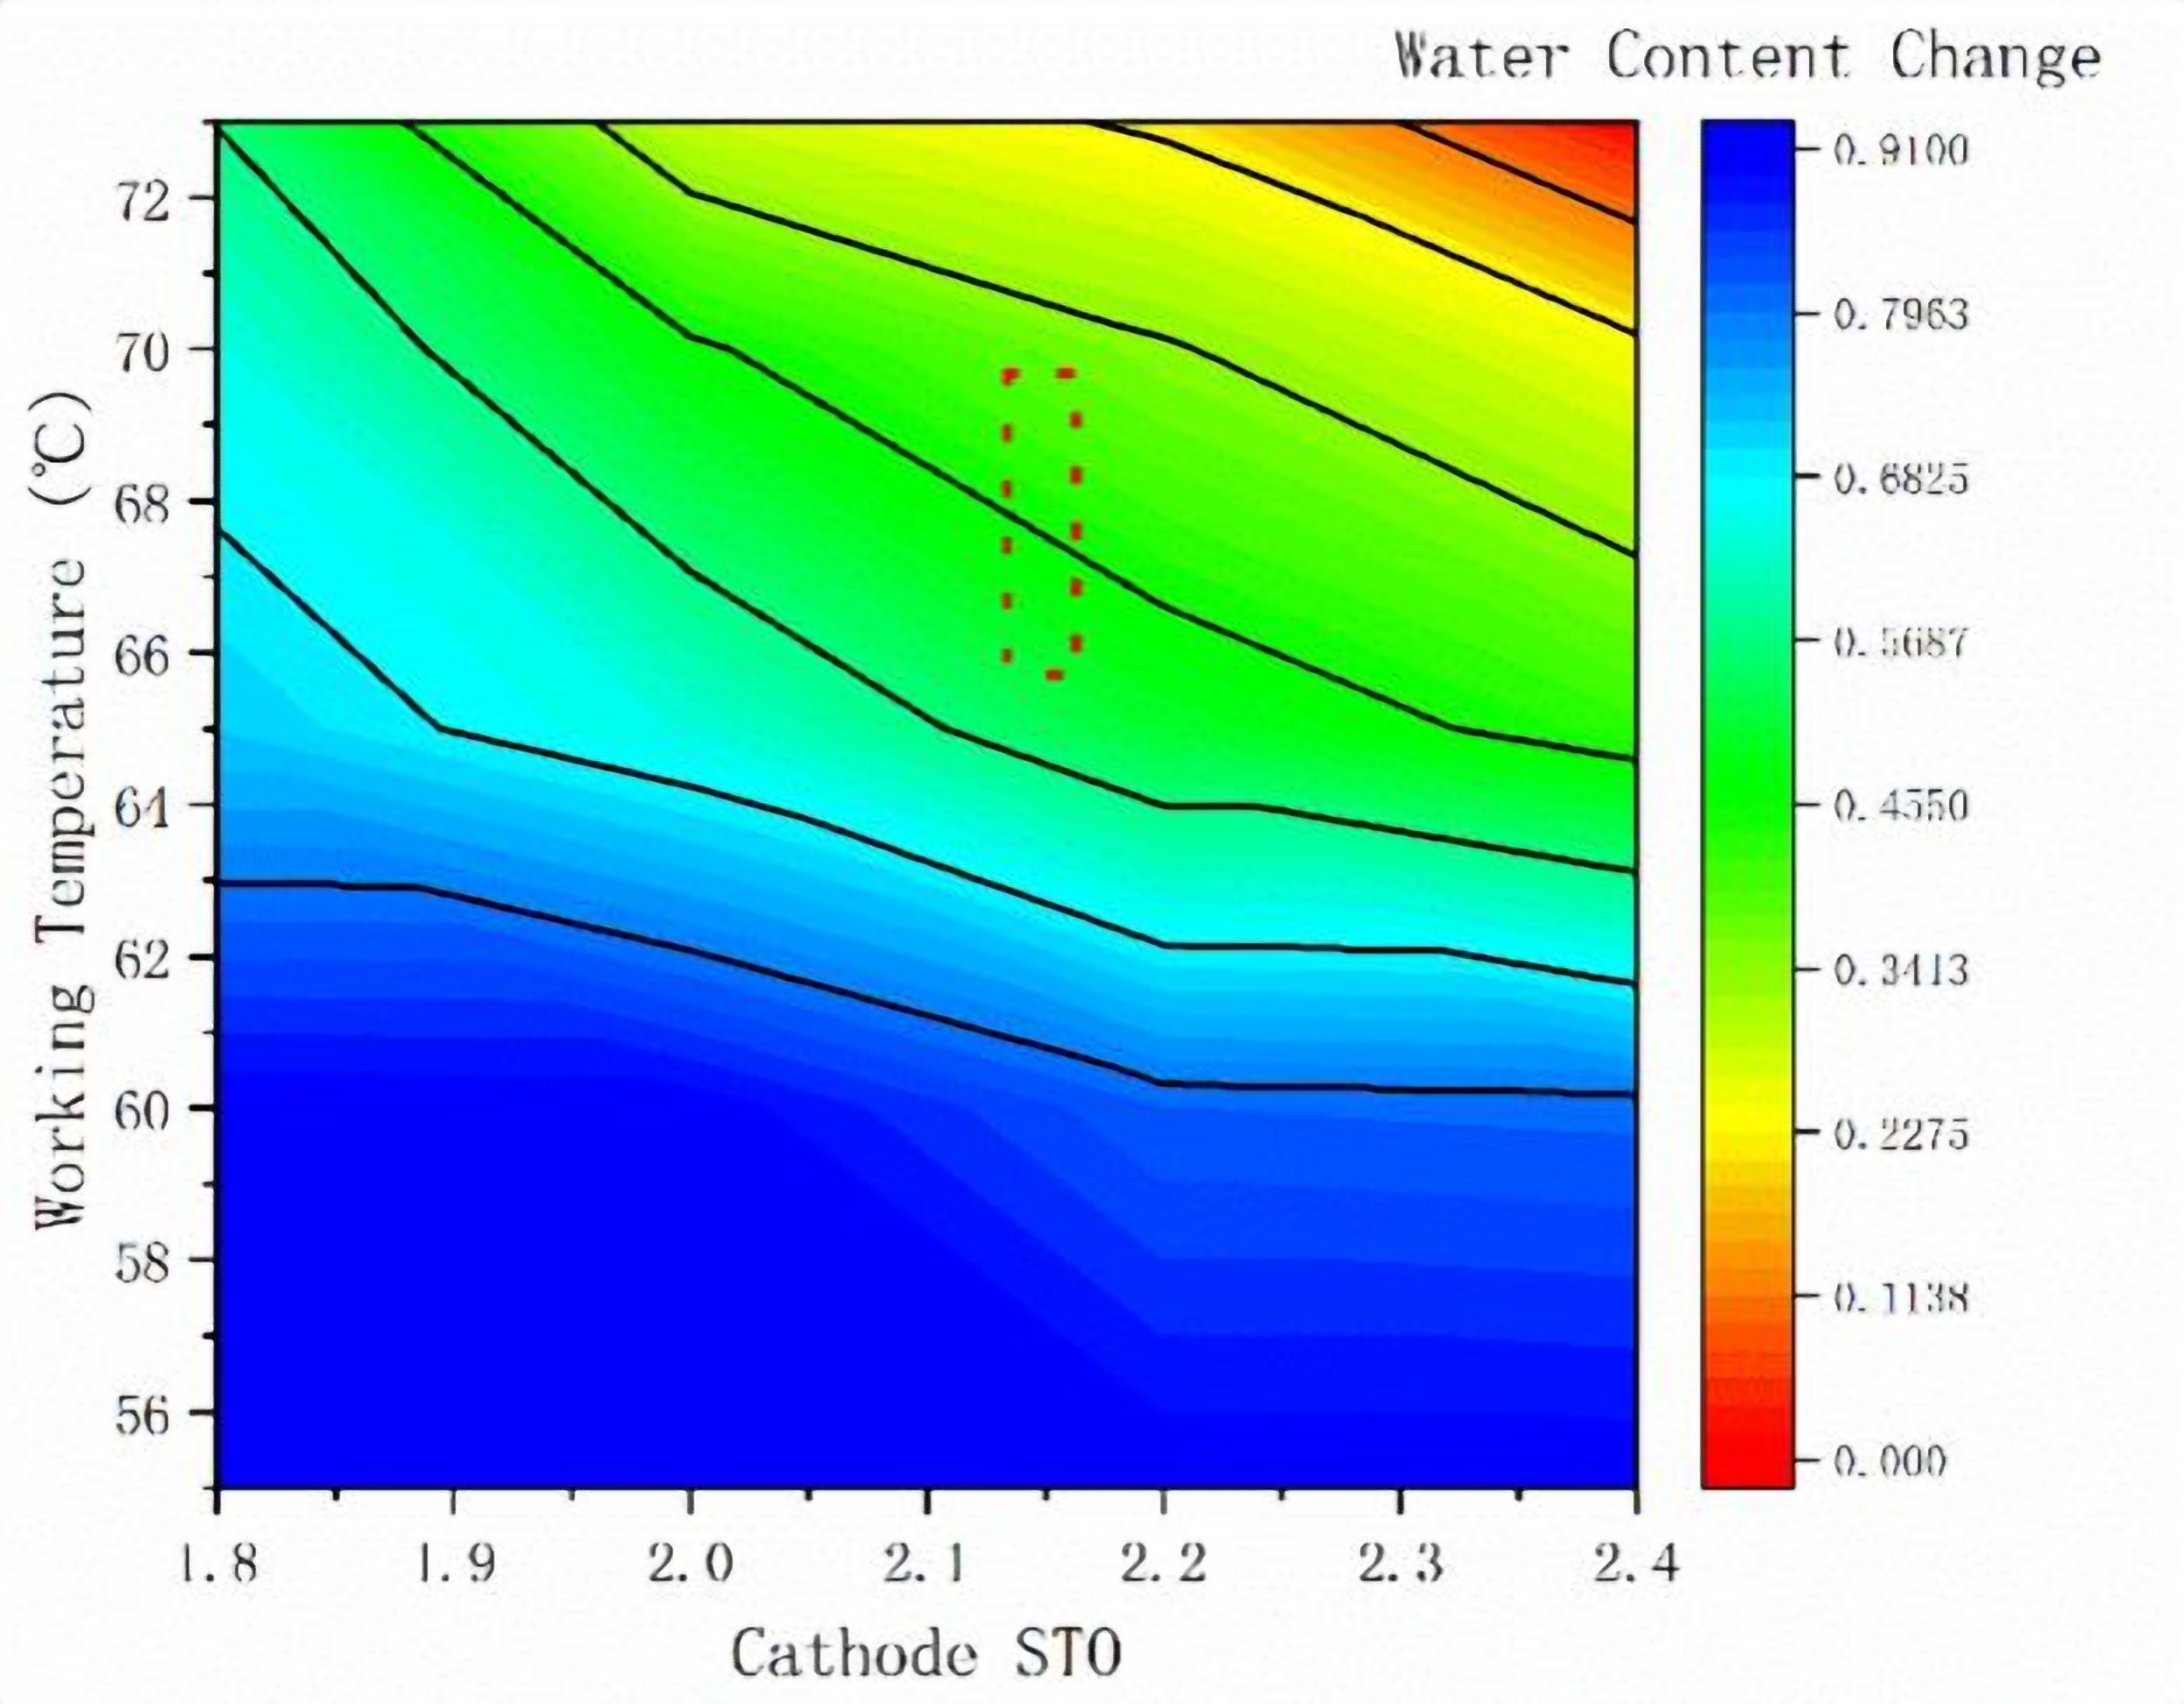
\includegraphics[width=0.5\textwidth]{Research_pictures/fig9b.jpg}}

	\subfloat[\label{fig:fig9c}]{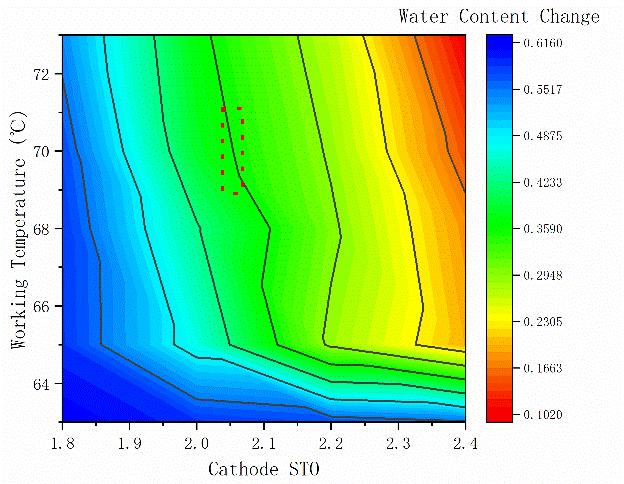
\includegraphics[width=0.5\textwidth]{Research_pictures/fig9c.jpg}}
	\caption{Selection of fuel cell OS operating environment (Working environment surrounded by dots, a:120A; b:210A; c:300A)}
	\label{fig:figure9}
\end{figure}
Next, comparing the rate of change of the water content inside the fuel cell system under different load currents.
% 接下来,比较不同负载电流下燃料电池系统内部含水量的变化率。

\begin{table}
	\centering
	\begin{center}
		\caption{Statistical table of the change rate of internal water content of different load currents}
		\label{tab:StatisticalTable}
		\begin{tabular}{l|c|c|c|c|r}
			\hline
			\textbf{Load current(A)} & \textbf{maximum} & \textbf{minimum} & \textbf{range} & \textbf{average} & \textbf{variance} \\
			\hline
			120                      & 0.342            & -0.177           & 0.519          & 0.086            & 0.019             \\
			210                      & 0.909            & 0.009            & 0.900          & 0.562            & 0.067             \\
			300                      & 0.615            & 0.103            & 0.512          & 0.402            & 0.028             \\
			\hline
		\end{tabular}
	\end{center}
\end{table}
From Table \ref{tab:StatisticalTable}, it can be seen that as the load current increases, the rate of change of the water content inside the fuel cell system increases to some extent, but the increase is not large. This may be because the higher the load current of the fuel cell, the more water flow is generated, so the water accumulated inside correspondingly increases. In addition, it was found that when the load current is 210A, the range is larger compared to 120A and 300A. Correspondingly, the fuel cell system cannot operate stably under the conditions of 210A/55$^{\circ}C$/1.6 and 210A/55$^{\circ}C$/1.8. This further reflects the connection between the rate of change of the internal water content of the fuel cell system and the water content fault.
% 从表\ref{tab:StatisticalTable}可以看出,随着负载电流的增加,燃料电池系统内部含水量的变化率有所增加,但增加幅度并不大。 这可能是因为燃料电池的负载电流越高,产生的水流就越多,因此内部积聚的水也相应增加。 另外发现,当负载电流为210A时,相比120A和300A,范围更大。 相应地,燃料电池系统在210A/55$^{\circ}C$/1.6和210A/55$^{\circ}C$/1.8条件下无法稳定运行。 这进一步体现了燃料电池系统内部含水量的变化率与含水量故障之间的联系。
\par
However, the above calculation method can only calculate the absolute value of the water content inside the fuel cell system. The output performance of the fuel cell in actual operation is related to the working temperature, intake pressure, and air metering ratio. To find the most suitable working conditions under each load current, it is necessary to establish a fuel cell stack model, and study the correlation between the difference between the actual output and theoretical output of the fuel cell stack under different conditions and the absolute value of the water content inside the fuel cell system.
% 然而,上述计算方法只能计算燃料电池系统内部水分含量的绝对值。 燃料电池在实际运行中的输出性能与工作温度、进气压力、空气计量比有关。 为了找到各负载电流下最适合的工况,需要建立燃料电池电堆模型,研究不同工况下燃料电池电堆的实际输出与理论输出的差值与绝对值之间的相关性。 燃料电池系统内的水含量。